 \documentclass[10pt,english]{beamer}
\usepackage{lmodern}
\usepackage[T1]{fontenc}
\usepackage[utf8]{inputenc}
\setcounter{tocdepth}{1}
\usepackage{amsbsy}
\usepackage{amstext}
\usepackage{amssymb}
\usepackage[authoryear]{natbib}

\makeatletter
%%%%%%%%%%%%%%%%%%%%%%%%%%%%%% Textclass specific LaTeX commands.
% this default might be overridden by plain title style
\newcommand\makebeamertitle{\frame{\maketitle}}%
% (ERT) argument for the TOC
\AtBeginDocument{%
  \let\origtableofcontents=\tableofcontents
  \def\tableofcontents{\@ifnextchar[{\origtableofcontents}{\gobbletableofcontents}}
  \def\gobbletableofcontents#1{\origtableofcontents}
}

%%%%%%%%%%%%%%%%%%%%%%%%%%%%%% User specified LaTeX commands.



\usepackage{tikz}
\usetikzlibrary{positioning}
\usepackage{appendixnumberbeamer}

\usepackage{graphicx}
\usepackage{subfig}

\usetheme[progressbar=frametitle,block=fill,subsectionpage=progressbar]{metropolis}

% margin
\setbeamersize{text margin right=1.5cm}

% colors
%\colorlet{DarkRed}{red!70!black}
\definecolor{DarkRed}{rgb}{0.7,0,0}

\setbeamercolor{normal text}{fg=black}
\setbeamercolor{alerted text}{fg=DarkRed}
\setbeamercolor{progress bar}{fg=DarkRed}
\setbeamercolor{button}{bg=DarkRed}

% width of seperators
\makeatletter
\setlength{\metropolis@titleseparator@linewidth}{1pt}
\setlength{\metropolis@progressonsectionpage@linewidth}{1pt}
\setlength{\metropolis@progressinheadfoot@linewidth}{1pt}
\makeatother

% new alert block
\newlength\origleftmargini
\setlength\origleftmargini\leftmargini
\setbeamertemplate{itemize/enumerate body begin}{\setlength{\leftmargini}{4mm}}
\let\oldalertblock\alertblock
\let\oldendalertblock\endalertblock
\def\alertblock{\begingroup \setbeamertemplate{itemize/enumerate body begin}{\setlength{\leftmargini}{\origleftmargini}} \oldalertblock}
\def\endalertblock{\oldendalertblock \endgroup}
\setbeamertemplate{mini frame}{}
\setbeamertemplate{mini frame in current section}{}
\setbeamertemplate{mini frame in current subsection}{}
\setbeamercolor{section in head/foot}{fg=normal text.bg, bg=structure.fg}
\setbeamercolor{subsection in head/foot}{fg=normal text.bg, bg=structure.fg}

% footer
\makeatletter
\setbeamertemplate{footline}{%
    \begin{beamercolorbox}[colsep=1.5pt]{upper separation line head}
    \end{beamercolorbox}
    \begin{beamercolorbox}{section in head/foot}
      \vskip1pt\insertsectionnavigationhorizontal{\paperwidth}{}{\hskip0pt plus1filll \insertframenumber{} / \inserttotalframenumber \hskip2pt}\vskip3pt%
    \end{beamercolorbox}%
    \begin{beamercolorbox}[colsep=1.5pt]{lower separation line head}
    \end{beamercolorbox}
}
\makeatother

% toc
\setbeamertemplate{section in toc}{\hspace*{1em}\inserttocsectionnumber.~\inserttocsection\par}
\setbeamertemplate{subsection in toc}{\hspace*{2em}\inserttocsectionnumber.\inserttocsubsectionnumber.~\inserttocsubsection\par}



% code
\usepackage{xcolor}
\usepackage{listings}

\definecolor{codegray}{rgb}{0.5,0.5,0.5}
\definecolor{background}{HTML}{F5F5F5}
\definecolor{keyword}{HTML}{4B69C6}
\definecolor{string}{HTML}{448C27}
\definecolor{comment}{HTML}{448C27}

\usepackage{inconsolata}
\lstdefinestyle{mystyle}{
    commentstyle=\color{comment},
    keywordstyle=\color{keyword},
    stringstyle=\color{string},
    basicstyle=\ttfamily,
    breakatwhitespace=false,
    breaklines=true,
    captionpos=b,
    keepspaces=true,
    numbersep=5pt,
    showspaces=false,
    showstringspaces=false,
    showtabs=false,
    tabsize=4,
	showlines=true
}

\lstset{style=mystyle}
% Added by lyx2lyx
\setlength{\parskip}{\smallskipamount}
\setlength{\parindent}{0pt}

\makeatother

\newcommand{\ikcdag}[2]{%
\begin{center}
\begin{tikzpicture}[blk/.style={draw,rounded corners=3pt,minimum width=21mm,minimum height=11mm,align=center,font=\small},lab/.style={font=\small,inner sep=2pt},ext/.style={font=\small,align=center,text=DarkRed},arr/.style={->,>=stealth,thick},scale=0.82,every node/.append style={transform shape}]
\node[ext] (sh) at (0,0) {Shock\\$\boldsymbol{r}$};
\node[blk] (go) at (2.6,0) {Government};
\node[blk,fill=DarkRed!20,draw=DarkRed,very thick] (hh) at (5.5,0) {#1\\#2};
\node[blk] (mc) at (8.4,0) {Goods market\\$\boldsymbol{Y}=\boldsymbol{C}+\boldsymbol{G}$};
\node[ext] (tg) at (10.9,0) {Target:\\goods};
\node[ext] (unk) at (6.95,1.75) {Unknown $\boldsymbol{Y}$};
\draw[arr] (sh)--(go);
\draw[arr] (go)--node[lab,above]{$\boldsymbol{T}$}(hh);
\draw[arr] (hh)--node[lab,above]{$\boldsymbol{C}$}(mc);
\draw[arr] (mc)--(tg);
\draw[arr] (unk)--(hh);
\draw[arr] (unk)--(mc);
\draw[arr] (sh.south)--(0,-1.5)--node[lab,below]{$\boldsymbol{r}$}(5.5,-1.5)--(hh.south);
\end{tikzpicture}
\end{center}}
\newcommand{\blockdag}[2]{%
\begin{center}
\begin{tikzpicture}[blk/.style={draw,rounded corners=3pt,minimum height=11mm,align=center,font=\small},lab/.style={font=\small,inner sep=2pt},ext/.style={font=\small,align=center,text=DarkRed},arr/.style={->,>=stealth,thick},scale=0.82,every node/.append style={transform shape}]
\node[ext] (unk) at (-0.2,0) {Unknowns\\$\boldsymbol{\pi}^{w},\boldsymbol{L}$};
\node[blk,dashed,inner sep=5pt] (ma) at (3.2,0) {\begin{tabular}{ll}Firms & $\boldsymbol{Y},\boldsymbol{\pi},\boldsymbol{d}$\\Central bank & $\boldsymbol{r}$\\Government & $\boldsymbol{\tau},\boldsymbol{T}$\\Mutual fund & $\boldsymbol{r}^{p}$\end{tabular}};
\node[blk,fill=DarkRed!20,draw=DarkRed,very thick] (hh) at (7.3,0) {#1\\#2};
\node[blk] (tg) at (10.9,0) {Goods market\\W-NKPC};
\node[ext] (sh) at (3.2,2.05) {Shocks $\boldsymbol{G},\boldsymbol{B},\boldsymbol{\epsilon}^{i}$};
\node[ext] (ok) at (10.9,-1.95) {Targets};
\draw[arr] (unk)--(ma);
\draw[arr] (sh)--(ma);
\draw[arr] (ma)--node[lab,above]{$\boldsymbol{Z},\boldsymbol{r}^{p}$}(hh);
\draw[arr] (hh)--node[lab,above]{$\boldsymbol{C}$}(tg);
\draw[arr] (tg)--(ok);
\draw[arr] (sh)-|node[lab,pos=0.25,above]{$\boldsymbol{G}$}(tg);
\draw[arr] (ma.south) |- node[lab,pos=0.75,below]{$\boldsymbol{Y},\boldsymbol{\pi}^{w},\boldsymbol{L},\boldsymbol{\tau}$} (9.9,-1.3)--(9.9,-0.56);
\end{tikzpicture}
\end{center}}

\usepackage{babel}
\begin{document}
\title{12. Monetary Policy in HANK, part 2\vspace{-2mm}}
\subtitle{Adv. Macro: Heterogeneous Agent Models}
\author{Raphaël Huleux}
\date{2026}

{
\setbeamertemplate{footline}{}
\begin{frame}

\maketitle

\end{frame}
}

\addtocounter{framenumber}{-1}

\section{Recap}

\begin{frame}{Second session}
\begin{itemize}
\item <+->\textbf{So far:}
\begin{itemize}
\item Monetary policy in RANK works mostly through intertemporal substitution (direct effect)
\item In HANK, mostly through the income feedback (indirect effect)
\item Same aggregate response in the benchmark (Werning, 2015)
\item The full model: capital gains, nominal bonds, unequal incidence
\end{itemize}
\item <+->\textbf{Now:} three extensions
\begin{enumerate}
\item Monetary policy works also by redistributing income (Auclert, 2019)
\item Dynamics: why is the data response hump-shaped?
\item Investment: why it matters more in HANK
\end{enumerate}
\end{itemize}
\end{frame}
%

\section{Auclert (2019)}

\begin{frame}{Motivation}
\begin{itemize}
\item <+->\textbf{Tobin (1982):}
\begin{quote}
\small Aggregation would not matter if we could be sure that the marginal propensities to spend from wealth were the same for creditors and for debtors. But {[}...{]} \textbf{the population is not distributed between debtors and creditors randomly. Debtors have borrowed for good reasons, most of which indicate a high marginal propensity to spend from wealth or from current income.}
\end{quote}
\item <+->A rate cut and surprise inflation move income and wealth across households
\item[$\Rightarrow$] <+-> What matters for aggregate demand: the \textbf{correlation between MPCs and who gains} from a monetary shock
\end{itemize}
\end{frame}
%
\begin{frame}{Auclert's decomposition}
\textbf{Part 1:} monetary policy = direct effect $\boldsymbol{M}^{r}d\boldsymbol{r}$ + indirect effect through aggregate income \\

\textbf{Auclert (2019)} splits the response of consumption on impact into two aggregate channels:


\begin{enumerate}
\item \textbf{Aggregate income:} the change in income, if each household received its usual share of it
\item \textbf{Substitution:} all unconstrained households change their consumption-saving plan
\end{enumerate}

and three redistribution channels:

\begin{enumerate}
\setcounter{enumi}{2}
\item \textbf{Earnings heterogeneity:} some households' earnings rise more than others'
\item \textbf{Fisher:} surprise inflation moves wealth from nominal savers to nominal debtors
\item \textbf{Interest rate exposure:} a rate cut hurts savers who reinvest at the lower rate, but stockholders get capital gains
\end{enumerate}

\end{frame}
%
\begin{frame}{Every Jacobian is a lump-sum Jacobian plus a covariance}
\begin{itemize}
\item <+->A household spends extra income the same way, \textbf{whatever its source}
\item <+->But different income flows go to different households: labor income in proportion to productivity, capital gains in proportion to wealth, a lump-sum transfer to everybody equally
\item <+->So the aggregate MPC out of each flow differs. A transfer $dx_{s}$ split with weights $\omega_{is}$, $\mathbb{E}[\omega_{is}]=1$:
\[
\frac{\partial C_{t}}{\partial x_{s}}=\mathbb{E}\left[\omega_{is}MPC_{i,t,s}\right]=\underbrace{\mathbb{E}[\omega_{is}]}_{=1}\underbrace{\mathbb{E}\left[MPC_{i,t,s}\right]}_{M_{t,s}^{\chi}}+\text{cov}\left(\omega_{is},MPC_{i,t,s}\right)
\]
\item <+->Lump-sum: $\omega_{is}=1$. Labor income: $\omega_{is}=z_{is}$, Wealth: $\omega_{i0}=a_{i,-1}/A_{ss}$.
\end{itemize}
\end{frame}
%
\begin{frame}{iMPCs by source of income}
\begin{figure}[H]
\centering
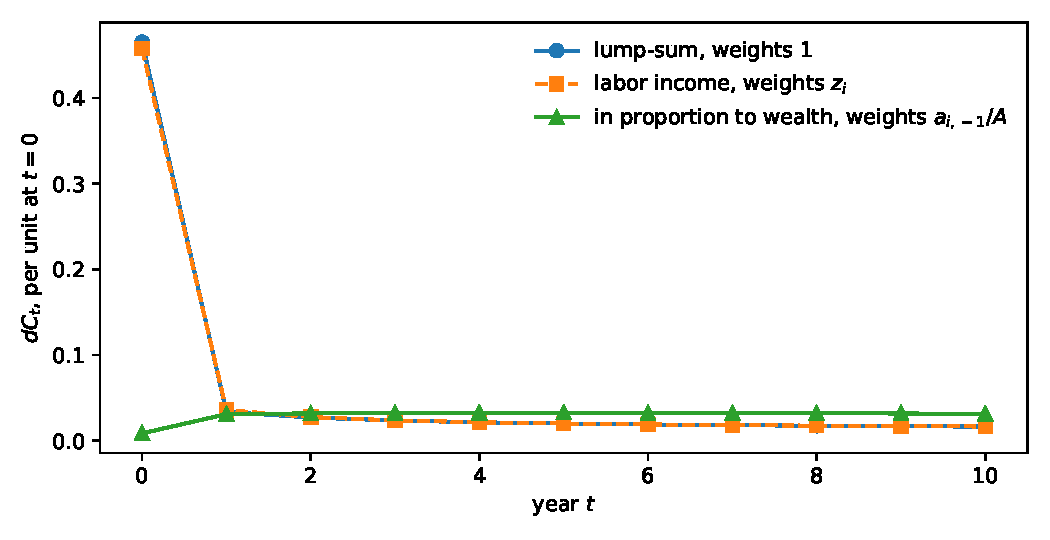
\includegraphics[width=\linewidth]{figs/iMPC_by_source.pdf}
\end{figure}

\end{frame}
%
\begin{frame}{Canonical HANK model}
\vspace{-1mm}
The full model of part 1 with two changes:
\begin{itemize}

\item[1.] <+->\textbf{Auclert's fiscal rule:} taxes are lump-sum, and the face value of debt is constant, $B_{t}=\frac{(1+r_{ss})B_{ss}}{1+r_{t}}$. The government rebates its gains at once:
\[
dT_{0}=B_{ss}dr_{0}^{b}+\frac{B_{ss}}{1+r_{ss}}dr_{0},\quad dT_{t}=\frac{B_{ss}}{1+r_{ss}}dr_{t}\text{ for }t\geq1
\]
with $dr_{0}^{b}\approx-(1+r_{ss})d\pi_{0}$ the surprise loss on nominal bonds
\item[2.] <+->\textbf{Unequal incidence on pre-tax labor income}, so tax changes no longer move inequality:
\[
c_{it}+a_{it}=(1+r_{t}^{p})a_{i,t-1}+Z_{t}\frac{z_{it}^{1+\zeta\log\left(Z_{t}/Z_{ss}\right)}}{\mathbb{E}\left[z_{it}^{1+\zeta\log\left(Z_{t}/Z_{ss}\right)}\right]}-T_{t},\quad Z_{t}=\frac{1}{\mu}Y_{t}
\]
\end{itemize}
\end{frame}
%
\begin{frame}{The household block}
\begin{itemize}
\item <+->Consumption responds to output, taxes, the surprise return at $t=0$, and the rate:
\[
d\boldsymbol{C}=\tfrac{1}{\mu}\tilde{\boldsymbol{M}}d\boldsymbol{Y}-\boldsymbol{M}^{\chi}d\boldsymbol{T}+\boldsymbol{m}\left(\text{cap}_{0}+B_{ss}dr_{0}^{b}\right)+\boldsymbol{M}^{r}d\boldsymbol{r}
\]
\item <+->Transfers, each $\boldsymbol{M}^{\chi}$ plus a covariance:
\begin{itemize}
\item $\boldsymbol{M}^{\chi}$: lump-sum transfer, weights $1$, and $\boldsymbol{m}^{\chi}$ its first column
\item $\boldsymbol{M}$: labor income with $\zeta=0$, weights $z_{is}$
\item $\tilde{\boldsymbol{M}}$: labor income with unequal incidence, weights $z_{is}+Z_{ss}\frac{\partial z_{is}}{\partial Z_{s}}$
\item $\boldsymbol{m}$: payment at $t=0$ in proportion to wealth, weights $\frac{a_{i,-1}}{A_{ss}}$
\end{itemize}
\item $\bar{\boldsymbol{M}}=\frac{1}{\mu}\boldsymbol{M}+\left(1-\frac{1}{\mu}\right)\boldsymbol{m}\boldsymbol{q}^{\prime}$, labor income and dividends with $\zeta=0$
\item The rate: $\boldsymbol{M}^{r}$. It combines:
\begin{itemize}
\item an income effect: a higher $r_{s}$ pays $a_{is}dr_{s}$
\item a substitution effect: saving pays more
\end{itemize}
\end{itemize}
\end{frame}
%
\begin{frame}{From the monetary IKC to Auclert}
\vspace{-1mm}
\begin{itemize}
\item <+->Replace $\text{cap}_{0}$ and $d\boldsymbol{T}$, and set $d\boldsymbol{Y}=d\boldsymbol{C}$:
{\small
\begin{align*}
d\boldsymbol{Y}= & \tfrac{1}{\mu}\tilde{\boldsymbol{M}}d\boldsymbol{Y}+\left(1-\tfrac{1}{\mu}\right)\boldsymbol{m}\boldsymbol{q}^{\prime}d\boldsymbol{Y}+B_{ss}\boldsymbol{m}dr_{0}^{b}-B_{ss}\boldsymbol{m}^{\chi}dr_{0}^{b}\\
 & +\boldsymbol{M}^{r}d\boldsymbol{r}-\tfrac{p}{1+r_{ss}}\boldsymbol{m}\boldsymbol{q}^{\prime}d\boldsymbol{r}-\tfrac{B_{ss}}{1+r_{ss}}\boldsymbol{M}^{\chi}d\boldsymbol{r}
\end{align*}
}
\item <+->Write $\tilde{\boldsymbol{M}}=\boldsymbol{M}+(\tilde{\boldsymbol{M}}-\boldsymbol{M})$ and group by shock:
{\small
\begin{align*}
d\boldsymbol{Y}= & \underbrace{\bar{\boldsymbol{M}}d\boldsymbol{Y}}_{\text{aggregate income}}+\underbrace{\tfrac{1}{\mu}(\tilde{\boldsymbol{M}}-\boldsymbol{M})d\boldsymbol{Y}}_{\text{earnings heterogeneity}}+\underbrace{B_{ss}\left(\boldsymbol{m}-\boldsymbol{m}^{\chi}\right)dr_{0}^{b}}_{\text{Fisher}}\\
 & +\underbrace{\left(\boldsymbol{M}^{r}-\tfrac{1}{1+r_{ss}}\left(p\,\boldsymbol{m}\boldsymbol{q}^{\prime}+B_{ss}\boldsymbol{M}^{\chi}\right)\right)d\boldsymbol{r}}_{\text{interest rate exposure and substitution}}
\end{align*}
}
\end{itemize}
\end{frame}
%
\begin{frame}{Auclert's decomposition of $dC_{0}$}
\vspace{-1mm}
\begin{itemize}
\item Focusing on $dY_{0}$ and using equation from slide 4,  we get
{\small
\begin{align*}
dC_{0}= & \underbrace{\mathbb{E}\left[\tfrac{Y_{i}}{Y}MPC_{i}\right]dY_{0}}_{\text{aggregate income}}+\underbrace{\text{cov}\left(MPC_{i},Z_{ss}dz_{i0}\right)}_{\text{earnings}}-\underbrace{\text{cov}\left(MPC_{i},NNP_{i}\right)d\pi_{0}}_{\text{Fisher}}\\
 & +\Big[\underbrace{\text{cov}\left(MPC_{i},URE_{i}\right)}_{\text{interest rate exposure}}-\underbrace{\tfrac{1}{\sigma}\mathbb{E}\left[\left(1-MPC_{i}\right)c_{i0}\right]}_{\text{substitution}}\Big]\frac{dr_{0}}{1+r_{ss}}
\end{align*}
}
\item <+->\textbf{Net nominal position:} $NNP_{i}=(1+r_{ss})\frac{B_{ss}}{A_{ss}}a_{i,-1}$,
\item <+->\textbf{Unhedged interest rate exposure:} $URE_{i}=a_{i0}-\frac{p}{A_{ss}}a_{i,-1}$ \\ what must be reinvested at the new rate.
\end{itemize}
\end{frame}
%
\begin{frame}{Auclert's result in the data (I)}

\begin{figure}[H]
\centering
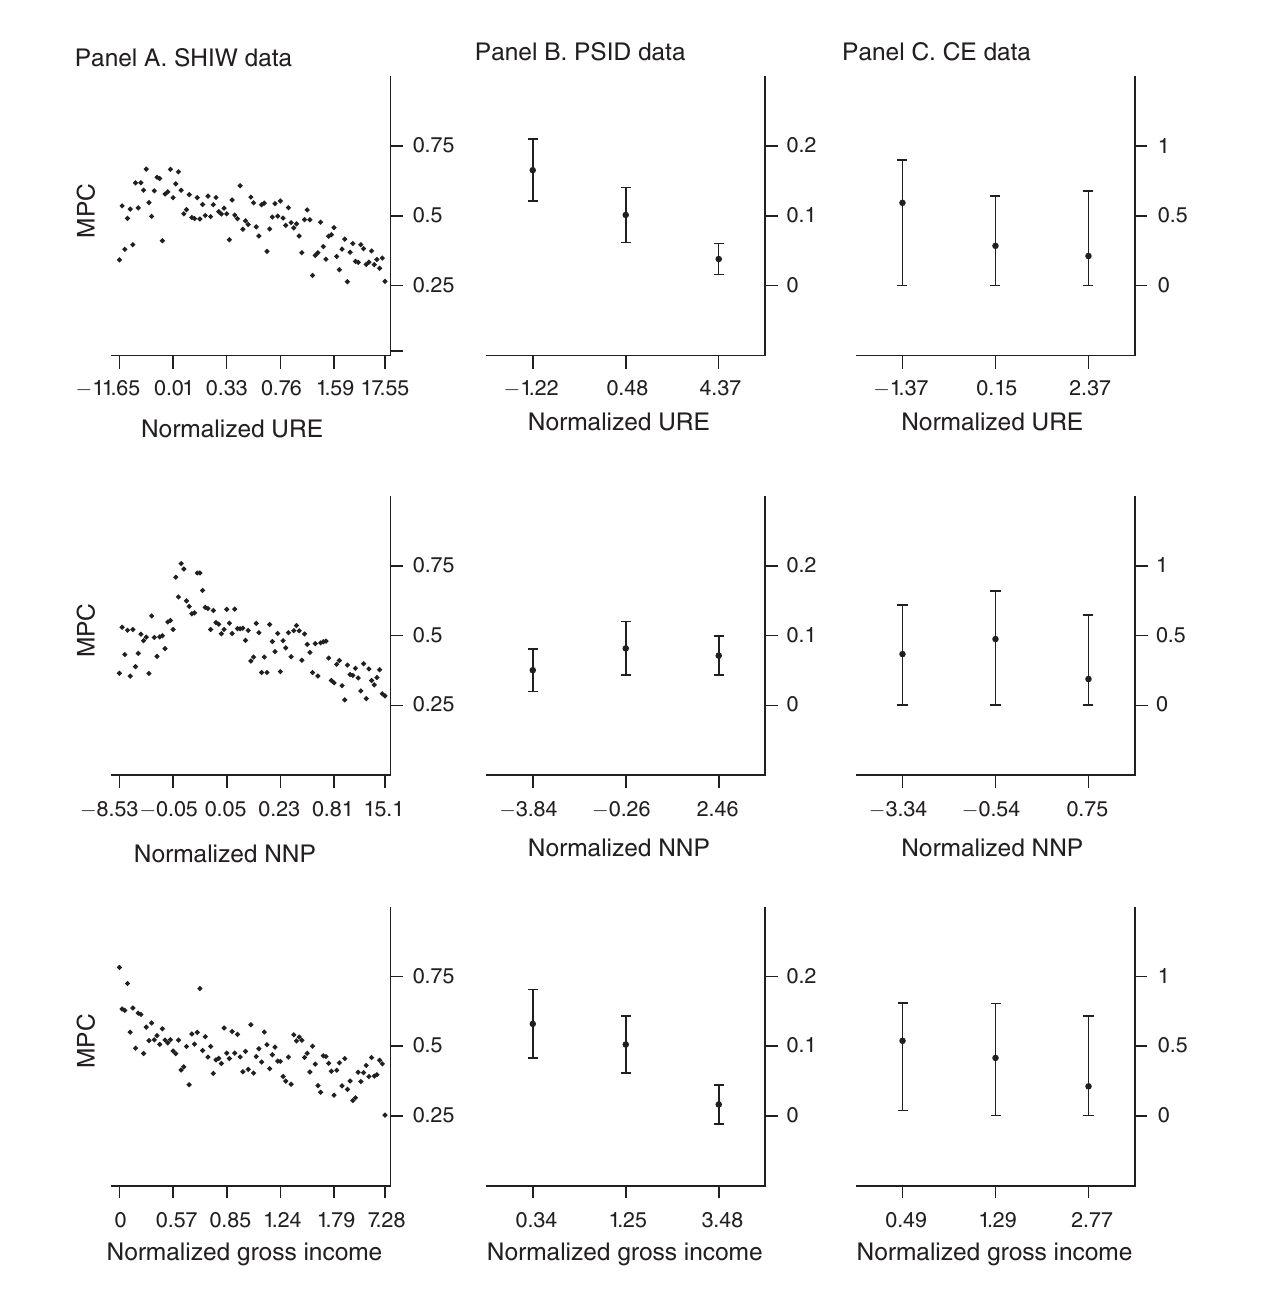
\includegraphics[height=0.55\textheight]{figs/AuclertFig2.png}
\end{figure}

$\Rightarrow$ MPCs fall with URE, NNP and income

\end{frame}
%
\begin{frame}{Auclert's result in the data (II)}
\begin{itemize}
\item <+->Sufficient statistics (Table 4), divided by $\mathbb{E}[c_{i}]$:
\begin{center}
\begin{tabular}{lccc}
 & SHIW & PSID & CE\tabularnewline
\hline
$\mathcal{E}_{R}=\text{cov}(MPC_{i},URE_{i})/C$ & $-0.10$ & $-0.12$ & $-0.23$\tabularnewline
$\mathcal{E}_{P}=\text{cov}(MPC_{i},NNP_{i})/C$ & $-0.07$ & $0.02$ & $-0.09$\tabularnewline
$S=\mathbb{E}[(1-MPC_{i})c_{i}]/C$ & $0.55$ & $0.90$ & $0.64$\tabularnewline
\end{tabular}
\end{center}
\item <+->Assuming a rate cut $\frac{dR}{R}=-1\%$ with inflation $\frac{dP}{P}=+1\%$, in \% of consumption:
\begin{itemize}
\item Interest rate exposure: $+0.10$ to $+0.23$
\item Fisher: $-0.02$ to $+0.09$
\item Substitution: $0.55$ to $0.90$ times the EIS of roughly $\leq 0.5$
\end{itemize}
\end{itemize}
$\Rightarrow$ The redistribution channels are of the same order as substitution, and amplify the rate cut
\end{frame}
%

\section[Micro Jumps]{Micro Jumps, Macro Humps}

\begin{frame}{Motivation}
\begin{itemize}
\item <+->Auclert, Rognlie and Straub (2020): estimate a HANK model on the causal effects of monetary policy
\item <+->\textbf{Micro:} consumption jumps after an income shock (iMPCs). \textbf{Macro:} $C$ and $Y$ respond with a hump\\
\begin{figure}[H]
\centering
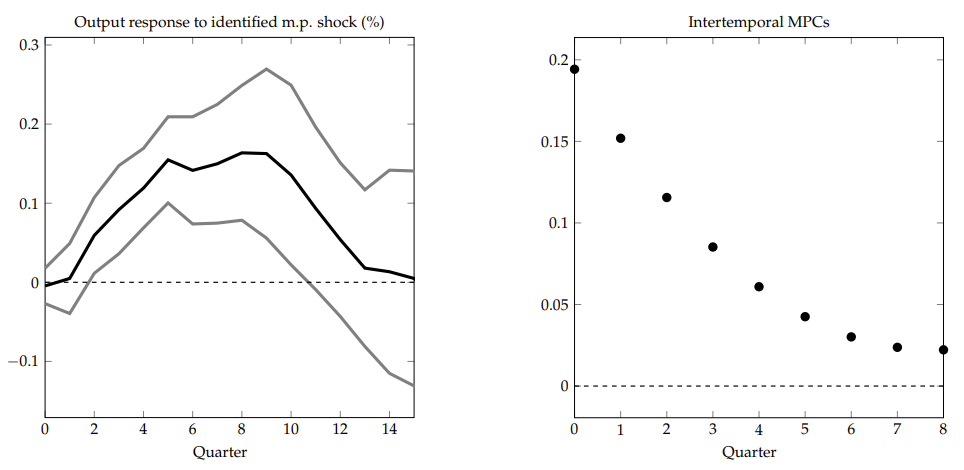
\includegraphics[width=0.55\linewidth]{figs/MJMCFig1.png}
\end{figure}
\item <+->\textbf{Standard HANK models cannot match this:} no hump, whatever the shape of the shock\\
\begin{figure}[H]
\centering
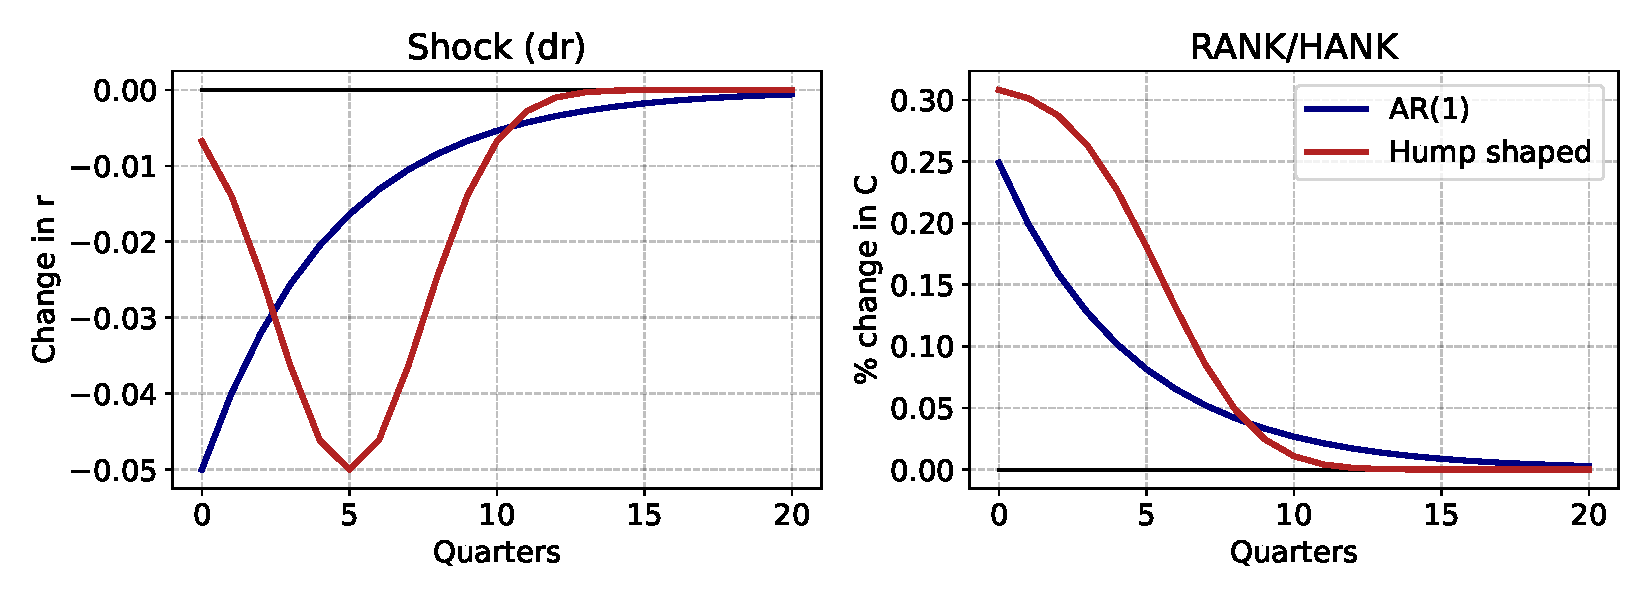
\includegraphics[width=0.6\linewidth]{figs/HANK_Monpol_shape.pdf}
\end{figure}
\end{itemize}
\end{frame}
%
\begin{frame}{The solution in RANK: habits}
\begin{itemize}
\item <+->Solution in the RANK literature: habits
\begin{align*}
\sum_{t=0}^{\infty} & \beta^{t}u\left(C_{t}-\gamma C_{t-1}\right)\\
\Rightarrow u'\left(C_{t}-\gamma C_{t-1}\right)= & \beta R_{t+1}u'\left(C_{t+1}-\gamma C_{t}\right)
\end{align*}
\item <+->Generates persistence: households do not want to deviate from last period's consumption
\item <+->\textbf{However:} does not work in HANK, because it kills the iMPCs\\
\begin{figure}[H]
\centering
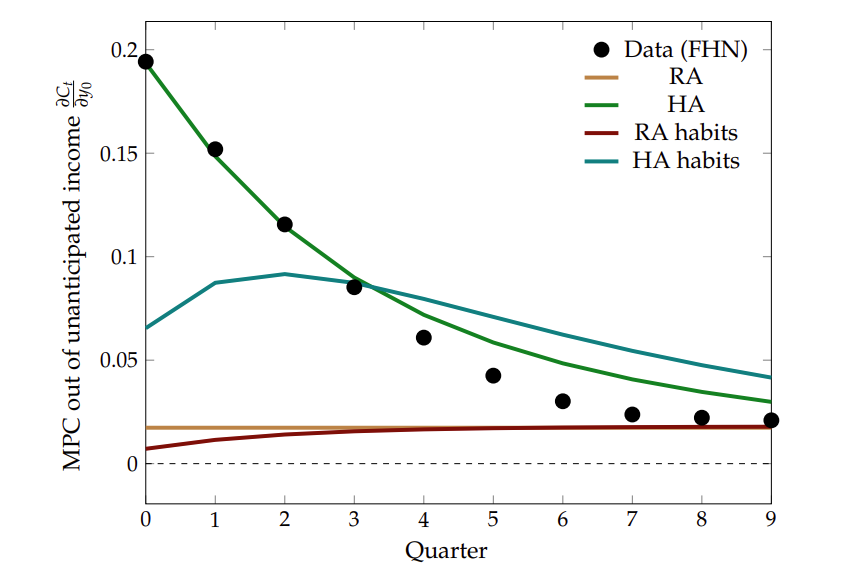
\includegraphics[width=0.5\linewidth]{figs/MJMCFig2.png}
\end{figure}
\end{itemize}
\end{frame}
%
\begin{frame}{Non-rational expectations in the sequence space}
\begin{itemize}
\item <+->\textbf{Solution:} deviate from rational expectations (RE)
\item <+->Households have imperfect expectations about \textbf{aggregates} ($Z,r$) only
\begin{itemize}
\item Steady state is unaffected
\item Still RE about idiosyncratic income shocks
\item First-order only: non-linear is much harder
\end{itemize}
\item <+->Take $d\boldsymbol{C}=\boldsymbol{M}d\boldsymbol{Z}$ under RE:
\[
\boldsymbol{M}=\begin{bmatrix}\frac{\partial C_{0}}{\partial Z_{0}} & \frac{\partial C_{0}}{\partial Z_{1}} & \frac{\partial C_{0}}{\partial Z_{2}} & \cdots\\
\frac{\partial C_{1}}{\partial Z_{0}} & \frac{\partial C_{1}}{\partial Z_{1}} & \frac{\partial C_{1}}{\partial Z_{2}} & \cdots\\
\frac{\partial C_{2}}{\partial Z_{0}} & \frac{\partial C_{2}}{\partial Z_{1}} & \frac{\partial C_{2}}{\partial Z_{2}} & \cdots\\
\vdots & \vdots & \vdots & \ddots
\end{bmatrix}
\]
\item <+->Only entries \textbf{above the diagonal} involve the future, so only they depend on expectations
\end{itemize}
\end{frame}
%
\begin{frame}{Expectations matrix}
\begin{itemize}
\item <+->Introduce the expectations matrix $\boldsymbol{E}$:
\[
\boldsymbol{E}=\begin{bmatrix}1 & * & * & * & \cdots\\
1 & 1 & * & * & \cdots\\
1 & 1 & 1 & * & \cdots\\
1 & 1 & 1 & 1 & \cdots\\
\vdots & \vdots & \vdots & \vdots & \ddots
\end{bmatrix}
\]
\item <+->$E_{t,s}$ is the average date-$t$ expectation about a shock to $Z$ at date $s$
\begin{itemize}
\item $E_{t,s}dZ_{s}$ is the expected value of $dZ_{s}$ at date $t$
\item First column: expectations at all dates about $dZ_{0}$
\item Second column: expectations at all dates about $dZ_{1}$
\end{itemize}
\item <+->How do we get the Jacobian $\hat{\boldsymbol{M}}$ implied by $\boldsymbol{E}$?
\end{itemize}
\end{frame}
%
\begin{frame}{Stylized example: myopic}
\begin{itemize}
\item <+->Myopic households only learn about a change in $Z$ when it happens: $\boldsymbol{E}=\left[\begin{smallmatrix}1 & 0 & 0 & \cdots\\
1 & 1 & 0 & \cdots\\
1 & 1 & 1 & \cdots\\
\vdots & \vdots & \vdots & \ddots
\end{smallmatrix}\right]$
\item <+->Each change in $Z$ is a surprise, so households react to it like to a shock at date 0:
\begin{align*}
d\hat{C}_{0} & =\frac{\partial C_{0}}{\partial Z_{0}}dZ_{0}\\
d\hat{C}_{1} & =\frac{\partial C_{1}}{\partial Z_{0}}dZ_{0}+\frac{\partial C_{0}}{\partial Z_{0}}dZ_{1}\\
d\hat{C}_{2} & =\frac{\partial C_{2}}{\partial Z_{0}}dZ_{0}+\frac{\partial C_{1}}{\partial Z_{0}}dZ_{1}+\frac{\partial C_{0}}{\partial Z_{0}}dZ_{2}
\end{align*}
\end{itemize}
\end{frame}
%
\begin{frame}{Myopic iMPCs}

\[
\boldsymbol{M}=\begin{bmatrix}\frac{\partial C_{0}}{\partial Z_{0}} & \frac{\partial C_{0}}{\partial Z_{1}} & \frac{\partial C_{0}}{\partial Z_{2}} & \cdots\\
\frac{\partial C_{1}}{\partial Z_{0}} & \frac{\partial C_{1}}{\partial Z_{1}} & \frac{\partial C_{1}}{\partial Z_{2}} & \cdots\\
\frac{\partial C_{2}}{\partial Z_{0}} & \frac{\partial C_{2}}{\partial Z_{1}} & \frac{\partial C_{2}}{\partial Z_{2}} & \cdots\\
\vdots & \vdots & \vdots & \ddots
\end{bmatrix},\quad\hat{\boldsymbol{M}}=\begin{bmatrix}\frac{\partial C_{0}}{\partial Z_{0}} & 0 & 0 & \cdots\\
\frac{\partial C_{1}}{\partial Z_{0}} & \frac{\partial C_{0}}{\partial Z_{0}} & 0 & \cdots\\
\frac{\partial C_{2}}{\partial Z_{0}} & \frac{\partial C_{1}}{\partial Z_{0}} & \frac{\partial C_{0}}{\partial Z_{0}} & \cdots\\
\vdots & \vdots & \vdots & \ddots
\end{bmatrix}
\]


\end{frame}
%
\begin{frame}{Intermediate version}
\vspace{-1mm}
\begin{itemize}
\item <+->Between RE and myopic, take $\boldsymbol{E}=\begin{bmatrix}1 & 0.4 & 0.3 & \cdots\\
1 & 1 & 0.6 & \cdots\\
1 & 1 & 1 & \cdots\\
\vdots & \vdots & \vdots & \ddots
\end{bmatrix}$
\item <+->Period 0: expected shocks are simply scaled
\[
d\hat{C}_{0}=\frac{\partial C_{0}}{\partial Z_{0}}dZ_{0}+0.4\frac{\partial C_{0}}{\partial Z_{1}}dZ_{1}+0.3\frac{\partial C_{0}}{\partial Z_{2}}dZ_{2}+\ldots
\]
\item <+->Period 1: {\footnotesize
\[
d\hat{C}_{1}=\underbrace{\frac{\partial C_{1}}{\partial Z_{0}}dZ_{0}}_{\text{Past shock}}+\underbrace{0.4\frac{\partial C_{1}}{\partial Z_{1}}dZ_{1}+\left(1-0.4\right)\frac{\partial C_{0}}{\partial Z_{0}}dZ_{1}}_{\text{Shock today}}+\underbrace{0.3\frac{\partial C_{1}}{\partial Z_{2}}dZ_{2}+\left(0.6-0.3\right)\frac{\partial C_{0}}{\partial Z_{1}}dZ_{2}}_{\text{Future shock}}
\]
}{\footnotesize\par}
\item <+->Past shock: fully known, standard effect
\item <+->Shock today: average of the forward-looking part and a myopic surprise
\item <+->Future shock: initial RE part plus the revision of expectations, weight $0.6-0.3$
\end{itemize}
\end{frame}
%
\begin{frame}{General formula}
\begin{itemize}
\item <+->General formula for $\hat{\boldsymbol{M}}$ given $\boldsymbol{E}$:
\[
\hat{M}_{t,s}=\sum_{\tau=0}^{\min\left\{ t,s\right\} }\underbrace{\left(E_{\tau,s}-E_{\tau-1,s}\right)M_{t-\tau,s-\tau}}_{\text{date-\ensuremath{t} effect of date-\ensuremath{\tau} revision about date-\ensuremath{s} shock}}
\]
\item <+->with $E_{-1,s}=0$ by convention
\item <+->\textbf{Fast} and \textbf{easy} to implement
\item <+->Solve general equilibrium with $\hat{\boldsymbol{M}},\hat{\boldsymbol{M}}^{r}$ in place of $\boldsymbol{M},\boldsymbol{M}^{r}$:
\[
d\boldsymbol{Y}=\hat{\boldsymbol{M}}\left(d\boldsymbol{Y}-d\boldsymbol{T}\right)+\hat{\boldsymbol{M}}^{r}d\boldsymbol{r}
\]
\end{itemize}
\end{frame}
%
\begin{frame}{Examples and Jacobians}
\vspace{-2mm}
\begin{itemize}
\item <+->Two extremes:{\footnotesize
\[
\boldsymbol{E}^{\text{RE}}=\begin{bmatrix}1 & 1 & 1 & \cdots\\
1 & 1 & 1 & \cdots\\
1 & 1 & 1 & \cdots\\
\vdots & \vdots & \vdots & \ddots
\end{bmatrix},\quad\boldsymbol{E}^{\text{Myopic}}=\begin{bmatrix}1 & 0 & 0 & \cdots\\
1 & 1 & 0 & \cdots\\
1 & 1 & 1 & \cdots\\
\vdots & \vdots & \vdots & \ddots
\end{bmatrix}
\]
}{\footnotesize\par}
\item <+->\textbf{Rational:} fully informed about the future path of $Z$ from the moment of the shock
\item <+->\textbf{Myopic:} not forward looking about aggregates, every change in $Z$ is a surprise\\
\begin{minipage}{0.42\textwidth}
\centering
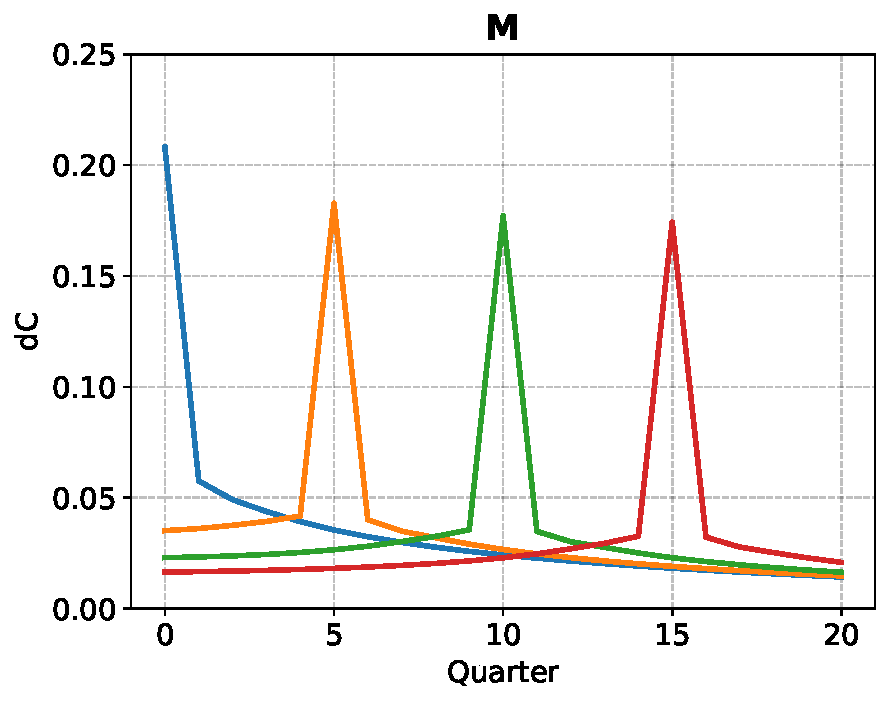
\includegraphics[width=\textwidth]{figs/M_RE.pdf}
\end{minipage}
\hfill
\begin{minipage}{0.42\textwidth}
\centering
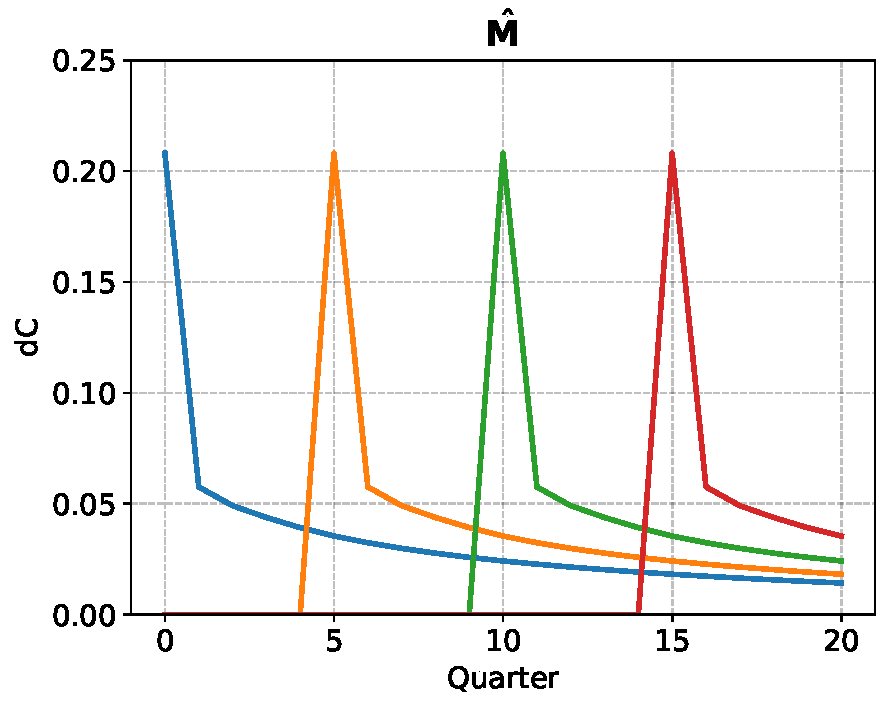
\includegraphics[width=\textwidth]{figs/M_myopic.pdf}
\end{minipage}
\end{itemize}
\end{frame}
%
\begin{frame}{Sticky expectations}
\begin{itemize}
\item <+->\textbf{Sticky information} (Mankiw and Reis, 2002): only a fraction $1-\theta$ of households update each period, and those learn the full path
\[
\boldsymbol{E}=\begin{pmatrix}1 & 1-\theta & 1-\theta & \dots\\
1 & 1 & 1-\theta^{2} & \dots\\
1 & 1 & 1 & \dots\\
\vdots & \vdots & \vdots & \ddots
\end{pmatrix}
\]
\item <+->Response of $C_{0}$ to $Z_{1}$: $\left(1-\theta\right)\frac{\partial C_{0}}{\partial Z_{1}}$
\item <+->Response of $C_{1}$ to $Z_{1}$: $\left(1-\theta\right)\frac{\partial C_{1}}{\partial Z_{1}}+\theta\frac{\partial C_{0}}{\partial Z_{0}}$
\item <+->$\theta=0$ is RE, $\theta=1$ is myopic
\item <+->Households observe income \textbf{today and in the past}, so iMPCs are preserved, unlike with habits
\end{itemize}
\end{frame}
%
\begin{frame}{Estimation and results (I)}
\begin{itemize}
\item <+->Full HANK with investment, sticky wages and prices, government, matched to Romer and Romer shocks
\item <+->Estimate $\theta=0.935$: a \textbf{large} deviation from RE\\
\begin{minipage}{0.46\textwidth}
\centering
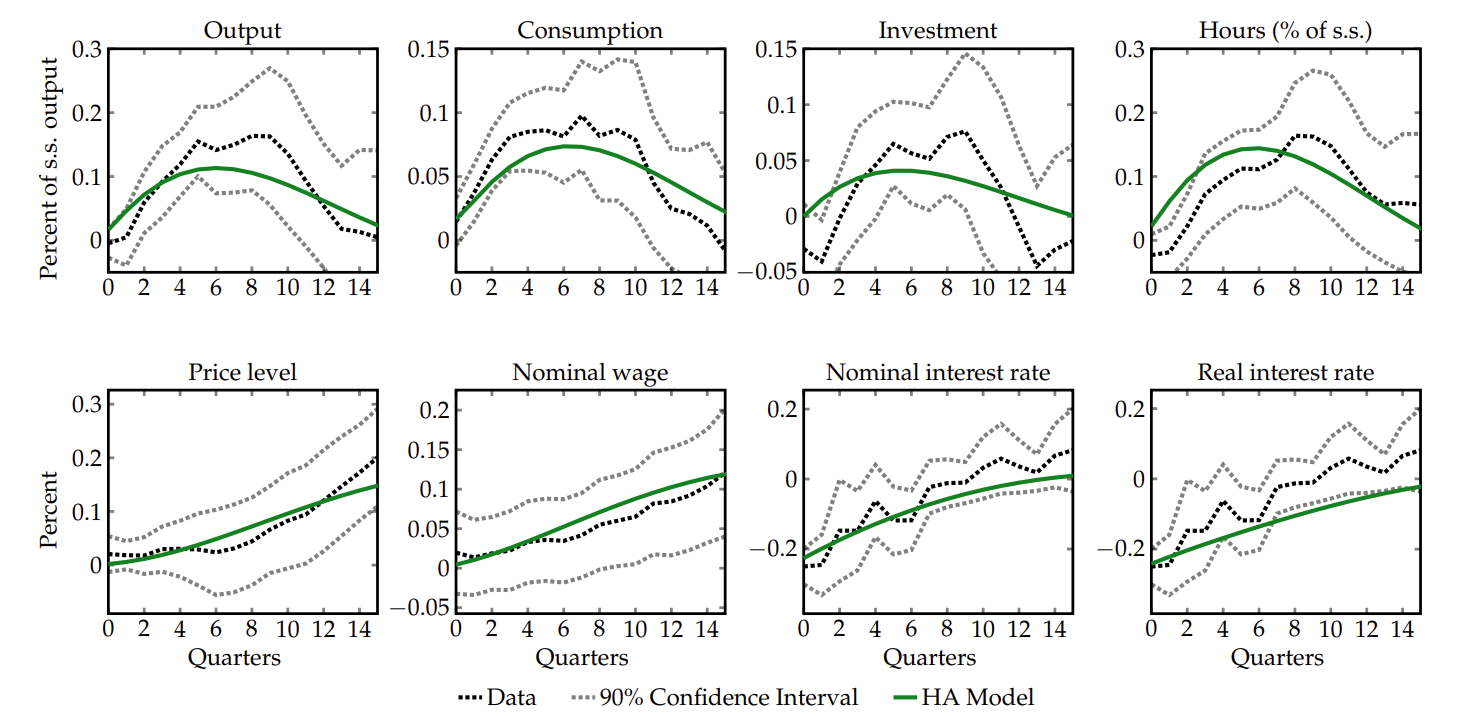
\includegraphics[width=\textwidth]{figs/MJMCFig3.png}
\end{minipage}
\hfill
\begin{minipage}{0.46\textwidth}
\centering
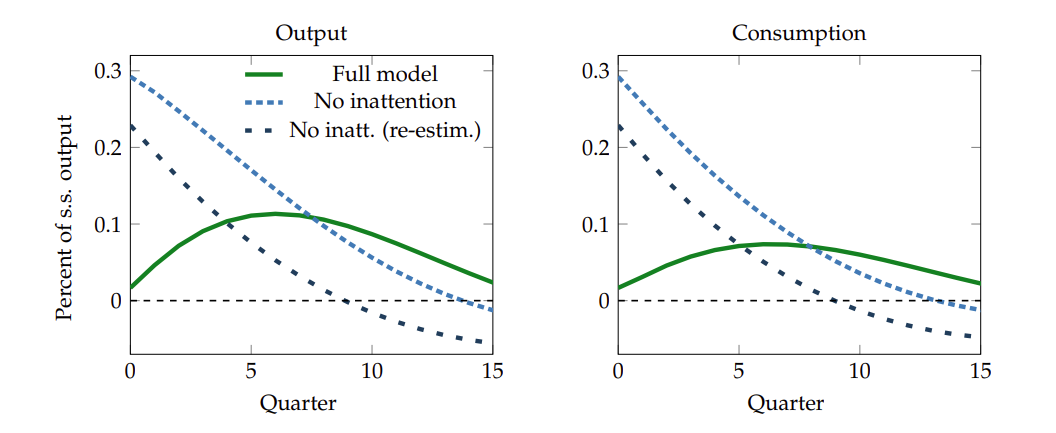
\includegraphics[width=\textwidth]{figs/MJMCFig4.png}
\end{minipage}
\item <+->Sticky expectations are needed to match the empirical response
\end{itemize}
\end{frame}
%
\begin{frame}{Estimation and results (II)}
\begin{itemize}
\item <+->Same decomposition as in the first session, in the estimated model\\
\begin{minipage}{0.46\textwidth}
\centering
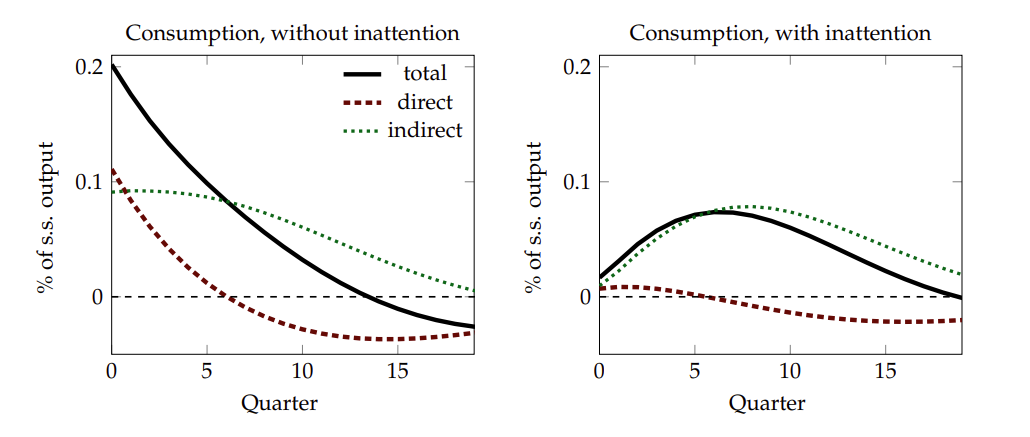
\includegraphics[width=\textwidth]{figs/MJMCFig6.png}
\end{minipage}
\hfill
\begin{minipage}{0.46\textwidth}
\centering
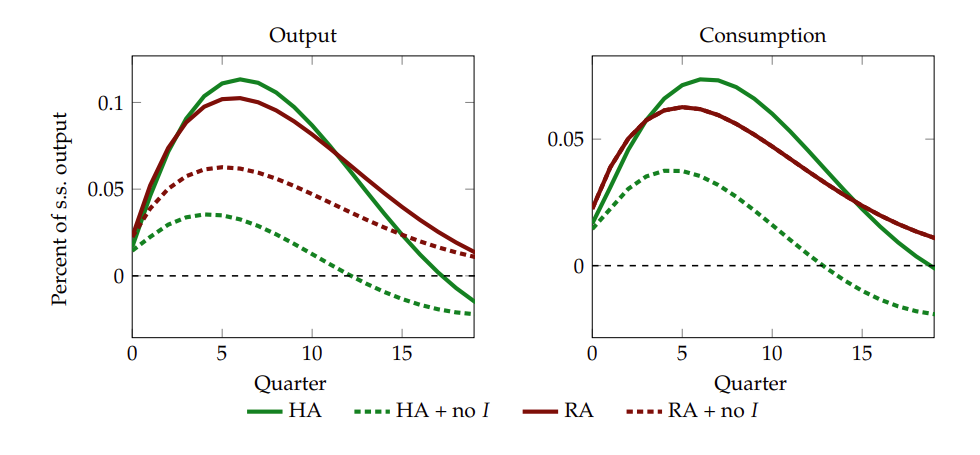
\includegraphics[width=\textwidth]{figs/MJMCFig5.png}
\end{minipage}
\item <+->With sticky expectations, the indirect effect is by far the main driver of consumption
\item <+->Part of it comes from \textbf{investment}: a channel missing from equivalence
\end{itemize}
\end{frame}
%
\section{Investment}

\begin{frame}{Intuition: IS-LM with investment}
\begin{itemize}
\item <+->\textbf{IS curve} $Y=C(Y,r)+I(Y,r)+G$, with the MPC $C_{Y}$, $I_{Y}>0$ (firms invest more when demand is high), $C_{r},I_{r}<0$. \textbf{LM:} the central bank sets $r$
\item <+->Rate shock $dr$:
\begin{align*}
dY & =C_{Y}dY+I_{Y}dY+(C_{r}+I_{r})dr\\
\Rightarrow\quad dY & =\underbrace{\frac{1}{1-C_{Y}-I_{Y}}}_{\text{multiplier}}\underbrace{(C_{r}+I_{r})dr}_{\text{direct effect}}
\end{align*}
\item <+->$r$ moves both $C$ and $I$. Investment adds to the direct effect ($I_{r}$) and raises the multiplier ($I_{Y}$)
\item <+->\textbf{RANK:} given $r$, the Euler equation pins down $C$, as if $C_{Y}=0$. Investment only adds its own demand
\item <+->\textbf{HANK:} high MPC $C_{Y}$. Investment raises income, households spend it, output rises further
\item <+->Later, the dynamic version: $C_{Y}\to\tilde{\boldsymbol{M}}$, $C_{r}\to\boldsymbol{M}^{r}$, $I_{Y}\to\boldsymbol{I}^{Y}$, $I_{r}\to\boldsymbol{I}^{r}$
\end{itemize}
\end{frame}
%
\begin{frame}{Investment in HANK: evidence}
\begin{itemize}
\item <+->Auclert, Rognlie and Straub (2020): investment is \textbf{the} transmission mechanism in their estimated HANK
\item <+->Shut off investment, holding the path of $r$ fixed:
\begin{itemize}
\item \textbf{HANK:} the peak output response shrinks by 69\%, and by 84\% cumulated over 5 years. For consumption: 49\% and 72\%
\item \textbf{RANK:} the output response shrinks by 38\%, the share of investment. Consumption does not move
\end{itemize}
\item <+->Why: as investment rises, labor income rises, high-MPC households spend it, and output rises further
\end{itemize}
\end{frame}

%
\begin{frame}{Changes to the model}
\begin{itemize}
\item <+->\textbf{Firms} now own physical capital and invest (next slides). Aggregate production, with $K_{t-1}$ installed at the end of $t-1$:
\[
Y_{t}=\Theta K_{t-1}^{\alpha}L_{t}^{1-\alpha},\qquad I_{t}=K_{t}-(1-\delta)K_{t-1}
\]
\item <+->\textbf{Dividends} now pay for investment and its adjustment cost:
\[
d_{t}=Y_{t}-w_{t}L_{t}-I_{t}-\phi\left(\tfrac{K_{t}}{K_{t-1}}\right)K_{t-1}
\]
\item <+->\textbf{Goods market:} investment is a new component of demand
\[
Y_{t}=C_{t}+G_{t}+I_{t}+\phi\left(\tfrac{K_{t}}{K_{t-1}}\right)K_{t-1}
\]
\item <+->\textbf{Unchanged:} sticky wages set by unions, households, mutual fund ($A_{t}=p_{t}+B_{t}$, $p_{t}=\frac{p_{t+1}+d_{t+1}}{1+r_{t}}$), government, central bank
\end{itemize}
\end{frame}
%
\begin{frame}{Firms: setup}
\vspace{-1mm}
\begin{itemize}
\item <+->\textbf{Final good producer:} competitive, aggregates intermediate goods $j\in[0,1]$
\[
Y_{t}=\left(\int_{0}^{1}y_{jt}^{\frac{1}{\mu}}dj\right)^{\mu}\quad\Rightarrow\quad y_{jt}=\left(\frac{P_{jt}}{P_{t}}\right)^{-\frac{\mu}{\mu-1}}Y_{t}
\]
\item <+->\textbf{Intermediate firm $j$:} monopolistic competition, flexible price $P_{jt}$, hires labor at $w_{t}$, owns its capital, with adjustment cost $\phi\left(\tfrac{K_{t}}{K_{t-1}}\right)=\frac{1}{2\delta\epsilon_{I}}\left(\tfrac{K_{t}}{K_{t-1}}-1\right)^{2}$
\item <+->Substitute demand into revenue, $\frac{P_{jt}}{P_{t}}y_{jt}=y_{jt}^{\frac{1}{\mu}}Y_{t}^{\frac{\mu-1}{\mu}}$, so firm $j$ only chooses $L_{jt}$ and $K_{jt}$, taking $Y_{t},w_{t},r_{t}$ as given:
{\small
\begin{align*}
J_{t}(K_{j,t-1})= & \max_{L_{jt},K_{jt}}\left[y_{jt}^{\frac{1}{\mu}}Y_{t}^{\frac{\mu-1}{\mu}}-w_{t}L_{jt}-I_{jt}-\phi\left(\tfrac{K_{jt}}{K_{j,t-1}}\right)K_{j,t-1}\right] +\frac{J_{t+1}(K_{jt})}{1+r_{t}}\\
\text{with}\quad & y_{jt}=\Theta K_{j,t-1}^{\alpha}L_{jt}^{1-\alpha},\qquad I_{jt}=K_{jt}-(1-\delta)K_{j,t-1}
\end{align*}
}
\end{itemize}
\end{frame}
%
\begin{frame}{Firms: optimality conditions}
\vspace{-1mm}
\begin{itemize}
\item <+->\textbf{First-order conditions}, then impose symmetry $y_{jt}=Y_{t}$, $K_{jt}=K_{t}$:
\begin{align*}
L_{jt}: & \ \tfrac{1}{\mu}y_{jt}^{\frac{1}{\mu}-1}Y_{t}^{\frac{\mu-1}{\mu}}\tfrac{(1-\alpha)y_{jt}}{L_{jt}}=w_{t}\quad\Rightarrow\quad w_{t}L_{t}=\tfrac{1-\alpha}{\mu}Y_{t}\\
K_{jt}: & \ 1+\phi^{\prime}\left(\tfrac{K_{t}}{K_{t-1}}\right)=\frac{J_{t+1}^{\prime}(K_{t})}{1+r_{t}}
\end{align*}
\item <+->\textbf{Envelope condition}, the value of one more unit of $K_{t}$ at $t+1$:
\[
J_{t+1}^{\prime}(K_{t})=\underbrace{\frac{\alpha}{\mu}\frac{Y_{t+1}}{K_{t}}}_{\text{marg. product}}+\underbrace{1-\delta}_{\text{saves inv.}}\underbrace{-\phi\left(\tfrac{K_{t+1}}{K_{t}}\right)+\tfrac{K_{t+1}}{K_{t}}\phi^{\prime}\left(\tfrac{K_{t+1}}{K_{t}}\right)}_{\text{lower adj. cost}}
\]
\item <+->\textbf{Combine} the last two into the capital condition:
\[
(1+r_{t})\left[1+\phi^{\prime}\left(\tfrac{K_{t}}{K_{t-1}}\right)\right]=\frac{\alpha}{\mu}\frac{Y_{t+1}}{K_{t}}+1-\delta-\phi\left(\tfrac{K_{t+1}}{K_{t}}\right)+\tfrac{K_{t+1}}{K_{t}}\phi^{\prime}\left(\tfrac{K_{t+1}}{K_{t}}\right)
\]
\item <+->\textbf{Steady state:} $\frac{K_{t}}{K_{t-1}}=1$, so $\phi=\phi^{\prime}=0$ and $1+r=\frac{\alpha}{\mu}\frac{Y}{K}+1-\delta$, hence $\frac{K}{Y}=\frac{\alpha}{\mu}\frac{1}{r+\delta}$ and $I=\delta K$
\end{itemize}
\end{frame}
%
\begin{frame}{Aggregate investment function}
\vspace{-1mm}
\begin{itemize}
\item <+->\textbf{Capital function:} given paths $\{Y_{s},r_{s}\}$, the capital condition is a second-order difference equation in $K$, with $K_{-1}$ given and $K_{t}\to K_{ss}$. One solution $K_{t}(\{Y_{s},r_{s}\})$ (ARS 2024, Lemma 5)
\item <+->\textbf{Investment function:} $I_{t}(\{Y_{s},r_{s}\})\equiv K_{t}(\{Y_{s},r_{s}\})-(1-\delta)K_{t-1}(\{Y_{s},r_{s}\})$. To first order
\[
d\boldsymbol{I}=\boldsymbol{I}^{Y}d\boldsymbol{Y}+\boldsymbol{I}^{r}d\boldsymbol{r},\qquad I_{t,s}^{Y}=\tfrac{\partial I_{t}}{\partial Y_{s}},\quad I_{t,s}^{r}=\tfrac{\partial I_{t}}{\partial r_{s}}
\]
\item <+->\textbf{Without adjustment costs} ($\epsilon_{I}\to\infty$, so $\phi=0$): $K_{t}=\frac{\alpha}{\mu}\frac{Y_{t+1}}{r_{t}+\delta}$, so $I_{t}=\frac{\alpha}{\mu}\frac{Y_{t+1}}{r_{t}+\delta}-(1-\delta)K_{t-1}$. Adjustment costs spread this response over time
\end{itemize}
\end{frame}
%
\begin{frame}{Investment Jacobians}
\begin{center}
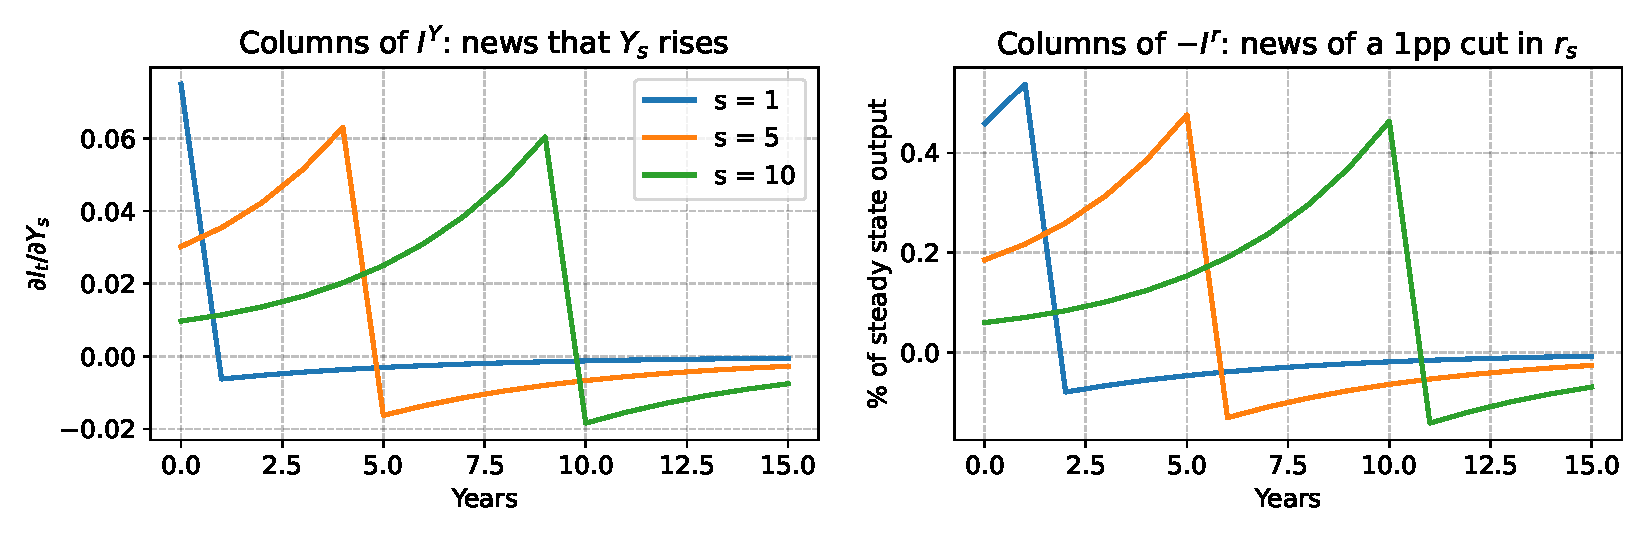
\includegraphics[width=\linewidth]{figs/inv_jacobians.pdf}
\par\end{center}

\end{frame}
%
\begin{frame}{The IKC with investment (I): households}
\vspace{-1mm}
\begin{itemize}
\item <+->\textbf{Household block unchanged}:
\[
d\boldsymbol{C}=\tfrac{1-\alpha}{\mu}{\boldsymbol{M}}d\boldsymbol{Y}-\boldsymbol{M}^{\chi}d\boldsymbol{T}+\boldsymbol{m}\left(\text{cap}_{0}+B_{ss}dr_{0}^{b}\right)+\boldsymbol{M}^{r}d\boldsymbol{r}
\]
\item <+->Two inputs change:
\begin{enumerate}
\item \textbf{Labor income} $w_{t}L_{t}=\frac{1-\alpha}{\mu}Y_{t}$, instead of $\frac{1}{\mu}Y_{t}$
\item \textbf{Dividends} are net of investment. To first order (adjustment costs are second order and disappear)
\[
dd_{t}=\left(1-\tfrac{1-\alpha}{\mu}\right)dY_{t}-dI_{t}
\]
\end{enumerate}
\item <+->\textbf{Capital gain}, as in part 1: $p_{0}+d_{0}$ is the present value of dividends, so
\begin{align*}
\text{cap}_{0}=d(p_{0}+d_{0}) & =\boldsymbol{q}^{\prime}d\boldsymbol{d}-\tfrac{p}{1+r_{ss}}\boldsymbol{q}^{\prime}d\boldsymbol{r}\\
 & =\left(1-\tfrac{1-\alpha}{\mu}\right)\boldsymbol{q}^{\prime}d\boldsymbol{Y}-\boldsymbol{q}^{\prime}d\boldsymbol{I}-\tfrac{p}{1+r_{ss}}\boldsymbol{q}^{\prime}d\boldsymbol{r}
\end{align*}
\item <+->Investment lowers the capital gain: shareholders pay for it
\item <+->$p$ now includes the value of the capital stock, $p=\frac{d}{r}$ with $d=\left(1-\frac{1-\alpha}{\mu}\right)Y-\delta K$
\end{itemize}
\end{frame}
%
\begin{frame}{The IKC with investment (II)}
\vspace{-1mm}
\begin{itemize}
\item <+->\textbf{Goods market}, to first order with $d\boldsymbol{G}=\boldsymbol{0}$: $d\boldsymbol{Y}=d\boldsymbol{C}+d\boldsymbol{I}$. Substitute $d\boldsymbol{C}$ and $\text{cap}_{0}$:
\begin{align*}
d\boldsymbol{Y}= & \tfrac{1-\alpha}{\mu}\tilde{\boldsymbol{M}}d\boldsymbol{Y}+\left(1-\tfrac{1-\alpha}{\mu}\right)\boldsymbol{m}\boldsymbol{q}^{\prime}d\boldsymbol{Y}-\boldsymbol{M}^{\chi}d\boldsymbol{T}+B_{ss}\boldsymbol{m}dr_{0}^{b}\\
 & +\left(\boldsymbol{M}^{r}-\tfrac{p}{1+r_{ss}}\boldsymbol{m}\boldsymbol{q}^{\prime}\right)d\boldsymbol{r}+\underbrace{(\mathrm{Id}-\boldsymbol{m}\boldsymbol{q}^{\prime})d\boldsymbol{I}}_{\text{new}}
\end{align*}
\item <+->Substitute $d\boldsymbol{I}=\boldsymbol{I}^{Y}d\boldsymbol{Y}+\boldsymbol{I}^{r}d\boldsymbol{r}$:
\begin{align*}
d\boldsymbol{Y}= & \left[\tfrac{1-\alpha}{\mu}\tilde{\boldsymbol{M}}+\left(1-\tfrac{1-\alpha}{\mu}\right)\boldsymbol{m}\boldsymbol{q}^{\prime}+(\mathrm{Id}-\boldsymbol{m}\boldsymbol{q}^{\prime})\boldsymbol{I}^{Y}\right]d\boldsymbol{Y}\\
 & +\left[\boldsymbol{M}^{r}-\tfrac{p}{1+r_{ss}}\boldsymbol{m}\boldsymbol{q}^{\prime}+(\mathrm{Id}-\boldsymbol{m}\boldsymbol{q}^{\prime})\boldsymbol{I}^{r}\right]d\boldsymbol{r}-\boldsymbol{M}^{\chi}d\boldsymbol{T}+B_{ss}\boldsymbol{m}dr_{0}^{b}
\end{align*}
\end{itemize}
\end{frame}

\begin{frame}{Investment in HANK: the feedback}
\begin{center}
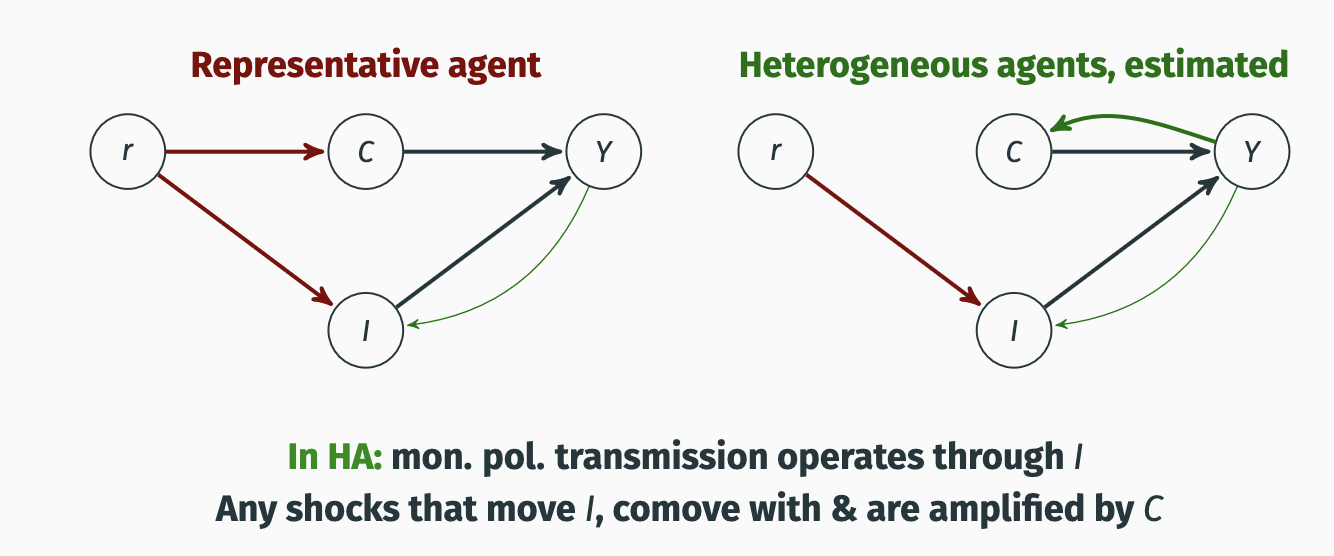
\includegraphics[width=0.95\linewidth]{figs/MJMH_feedback.png}
\par\end{center}
{\footnotesize Source: Auclert, Rognlie and Straub (2020).}
\begin{itemize}
\item <+->\textbf{This section:} add investment to our canonical HANK model, as in Auclert, Rognlie and Straub (2024, section 7 and appendices B.6, G.1)
\end{itemize}
\end{frame}

\begin{frame}{Research frontier: heterogeneous households and firms}
\begin{itemize}
\item <+->So far: heterogeneous households, representative firm. Investment depends on $Y$ and $r$, not on cash flow
\item <+->\textbf{Ottonello and Winberry (2020):} heterogeneous firms with default risk. The investment response to monetary policy depends on leverage: low-leverage firms respond the most
\item <+->\textbf{Winberry, Auclert, Rognlie and Straub (2025):} the HANK lessons carry over to firms
\begin{itemize}
\item Constrained firms have a positive \textbf{marginal propensity to invest} (MPI) out of cash flow, like the MPC
\item Monetary policy gets indirect effects through cash flows (about 15\% of the investment response)
\item Deficit-financed transfers to firms raise investment
\item Complementarity with high-MPC households: about 20\% of the effect of a transfer to firms
\end{itemize}
\item <+->Open question: no quasi-experimental estimates of MPIs yet, unlike MPCs
\end{itemize}
\end{frame}
%

\section{Summary}

\begin{frame}{Summary and next week}
\begin{itemize}
\item <+->\textbf{HANK for fiscal policy:} multipliers change
\item <+->\textbf{HANK for monetary policy:} the mechanism changes
\item <+->\textbf{Next week:} open economy and unemployment risk
\end{itemize}
\end{frame}
%

\section{Exercise}

\begin{frame}{Exercises: second session}
\begin{enumerate}
\item <+->Solve for a monetary policy shock in HANK and RANK with myopic expectations w.r.t. $\boldsymbol{r},\boldsymbol{Z}$, only $\boldsymbol{r}$ and only $\boldsymbol{Z}$
\item <+->Do the same with sticky expectations
\item <+->Compare with rational expectations. Which case gives a hump in $C$?
\end{enumerate}
\end{frame}
%
\begin{frame}{Non-RE in GEModelTools}
\begin{itemize}
\item <+->No built-in way, so a workaround (see exercise):
\begin{enumerate}
\item <+->Compute all household Jacobians: \lstinline{model._compute_jac_hh()}
\item <+->Construct $\boldsymbol{E}$ and compute $\hat{\boldsymbol{M}}$ from the RE Jacobians in \lstinline{model.jac_hh}
\item <+->Overwrite \lstinline{model.jac_hh} with $\hat{\boldsymbol{M}}$ for each output and input of the household block
\item <+->Compute Jacobians with respect to unknowns and shocks, but \textbf{not} the household block: \lstinline{model.compute_jacs(skip_hh=True,skip_shocks=False)}
\item <+->Solve for IRFs: \lstinline{model.find_IRFs(shocks=[x])}
\end{enumerate}
\end{itemize}
\end{frame}
%


\end{document}
